%        File: arfc-beamer.tex
%     Created: Sun May 5 10:00 PM 2013 C
%


%\documentclass[11pt,handout]{beamer}
\documentclass[9pt]{beamer}
\usetheme[white]{Illinois}
\title[Short Title]{Demand Driven Deployment Capabilities in \Cyclus}
\author[Your Name]{Gwendolyn J. Chee$^1$, Roberto E. Fairhurst Agosta$^1$, Jin Whan Bae$^2$, Robert R. Flanagan$^3$, and Kathryn D. Huff$^1$}
\date[09.24.2019]{September 24, 2019}
\institute{
$^1$Dept. of Nuclear, Plasma and Radiological Engineering, University of Illinois at Urbana-Champaign \\
$^2$ Oak Ridge National Laboratory, Oak Ridge, TN, United States \\
$^3$Nuclear Engineering Program, University of South Carolina \\
}

%\usepackage{bbding}
\usepackage{amsfonts}
\usepackage{amsmath}
\usepackage{xspace}
\usepackage{graphicx}
\usepackage{booktabs} % nice rules for tables
\usepackage{microtype} % if using PDF
\usepackage{bigints}
\usepackage{minted}
\usepackage{subfigure}

\newcommand{\Cyclus}{\textsc{Cyclus}\xspace}%
\newcommand{\Cycamore}{\textsc{Cycamore}\xspace}%
\newcommand{\deploy}{\texttt{d3ploy}\xspace}%
\newcommand{\units}[1] {\:\text{#1}}%
\newcommand{\SN}{S$_N$}%{S$_\text{N}$}%{$S_N$}%
\DeclareMathOperator{\erf}{erf}
%I need some complimentary error funcitons... 
\DeclareMathOperator{\erfc}{erfc}
%page numbers
\setbeamertemplate{footline}[page number]
\setbeamertemplate{caption}[numbered]
%Those icons in the references are terrible looking
\setbeamertemplate{bibliography item}[text]

\usepackage{tikz}
\usetikzlibrary{positioning, arrows, decorations, shapes}

\usetikzlibrary{shapes.geometric,arrows}
\tikzstyle{process} = [rectangle, rounded corners, minimum width=3cm, minimum height=1cm,text centered, draw=black, fill=blue!30]
\tikzstyle{object} = [ellipse, rounded corners, minimum width=3cm, minimum height=1cm,text centered, draw=black, fill=green!30]
\tikzstyle{arrow} = [thick,->,>=stealth]

\definecolor{illiniblue}{HTML}{B1C6E2}
\definecolor{illiniorange}{HTML}{f8c2a2}
\usetikzlibrary{shapes.geometric, arrows}
\tikzstyle{oblock} = [rectangle, draw, fill=illiniorange, 
text width=15em, text centered, rounded corners, minimum height=4em]
\tikzstyle{bblock} = [rectangle, draw, fill=illiniblue, 
text width=15em, text centered, rounded corners, minimum height=4em]
\tikzstyle{arrow} = [thick,->,>=stealth]

\usepackage{tabularx}
\newcolumntype{b}{>{\hsize=1.0\hsize}X}
\newcolumntype{s}{>{\hsize=.5\hsize}X}
\newcolumntype{m}{>{\hsize=.75\hsize}X}
\newcolumntype{x}{>{\hsize=.25\hsize}X}
\newcolumntype{L}{>{\raggedright\arraybackslash}X}
\newcolumntype{R}{>{\raggedleft\arraybackslash}X}
\def\arraystretch{1}
%%%% Acronym support
\usepackage{multirow}
\usepackage{graphicx,subfigure}

\usepackage[acronym,toc]{glossaries}
\include{acros}

\makeglossaries

%try to get rid of header on title page\dots
\makeatletter
    \newenvironment{withoutheadline}{
        \setbeamertemplate{headline}[default]
        \def\beamer@entrycode{\vspace*{-\headheight}}
    }{}
\makeatother

% add slide numbers
\makeatother
\setbeamertemplate{footline}
{
  \leavevmode%
  \hbox{%
    \rightline{\insertframenumber{} / \inserttotalframenumber\hspace*{1ex}}
  }%
  \vskip0pt%
}
\makeatletter

\begin{document}
%%%%%%%%%%%%%%%%%%%%%%%%%%%%%%%%%%%%%%%%%%%%%%%%%%%%%%%%%%%%%
%% From uw-beamer Here's a handy bit of code to place at 
%% the beginning of your presentation (after \begin{document}):
\newcommand*{\alphabet}{ABCDEFGHIJKLMNOPQRSTUVWXYZabcdefghijklmnopqrstuvwxyz}
\newlength{\highlightheight}
\newlength{\highlightdepth}
\newlength{\highlightmargin}
\setlength{\highlightmargin}{2pt}
\settoheight{\highlightheight}{\alphabet}
\settodepth{\highlightdepth}{\alphabet}
\addtolength{\highlightheight}{\highlightmargin}
\addtolength{\highlightdepth}{\highlightmargin}
\addtolength{\highlightheight}{\highlightdepth}
\newcommand*{\Highlight}{\rlap{\textcolor{HighlightBackground}{\rule[-\highlightdepth]{\linewidth}{\highlightheight}}}}
%%%%%%%%%%%%%%%%%%%%%%%%%%%%%%%%%%%%%%%%%%%%%%%%%%%%%%%%%%%%%
%%--------------------------------%%
\begin{withoutheadline}
\frame{
  \titlepage
}
\end{withoutheadline}

%%--------------------------------%%
\AtBeginSection[]{
\begin{frame}
  \frametitle{Outline}
  \tableofcontents[currentsection]
\end{frame}
}

\section{Background and Motivation}
\subsection{Cyclus}
\begin{frame}
    \frametitle{Cyclus}
        \texttt{Cyclus} is an agent-based nuclear fuel cycle simulator with a modular architecture.
        It has three types of agents: \texttt{Facility}, \texttt{Institution}, and \texttt{Region}.
     \\   
    \begin{figure}[htbp!]
      \begin{center}
        \includegraphics[height=4.5cm]{../paper/figures/nfc}
      \end{center}
            \caption{Once Through Nuclear Fuel Cycle \cite{huff_fundamental_2016}}
      \label{fig:cyclus-modular}
    \end{figure}
  \end{frame}
  
\input{validation}
\subsection{Goal}
\begin{frame}
    \frametitle{Goals}
    \textbf{Goals of this work} 
    \begin{itemize}
        \item Develop demand driven deployment capabilities in \Cyclus (\deploy)
        \item Demonstrate the use of \deploy to set up transition scenarios 
        from the current once through \gls{LWR} fuel cycle to four other more 
        promising fuel cycles. 
    \end{itemize}

    \begin{table}[]
        \centering
        \caption{Descriptions of the current and other high performing nuclear fuel cycle evaluation groups described in the evaluation and screening study \cite{wigeland_nuclear_2014}.}
        \label{tab:eg}
            \footnotesize
            \begin{tabularx}{\textwidth}{l|lll}
                \hline
            \textbf{Fuel Cycle}                                               & \textbf{Open or Closed} & \textbf{Fuel Type}                                                              & \textbf{Reactor Type}                                                                           \\ \hline
            \textbf{\begin{tabular}[c]{@{}l@{}}EG01\\ (current)\end{tabular}} & Open                                                               & Enriched-U                                                                      & Thermal critical reactors                                                                       \\ 
            \textbf{EG23}                                                     & Closed                                                             & \begin{tabular}[c]{@{}l@{}}Recycle of U/Pu \\ with natural-U fuel\end{tabular}  & Fast critical reactors                                                                          \\ 
            \textbf{EG24}                                                     & Closed                                                             & \begin{tabular}[c]{@{}l@{}}Recycle of U/TRU \\ with natural-U fuel\end{tabular} & Fast critical reactors                                                                          \\ 
            \textbf{EG29}                                                     & Closed                                                             & \begin{tabular}[c]{@{}l@{}}Recycle of U/Pu \\ with natural-U fuel\end{tabular}  & \begin{tabular}[c]{@{}l@{}}Fast critical reactors and \\ thermal critical reactors\end{tabular} \\ 
            \textbf{EG30} & Closed                                                             & \begin{tabular}[c]{@{}l@{}}Recycle of U/TRU \\ with natural-U fuel\end{tabular} & \begin{tabular}[c]{@{}l@{}}Fast critical reactors and \\ thermal critical reactors\end{tabular} \\ \hline
        \end{tabularx}
    \end{table}

\end{frame}
%\input{validation}

\section{Method}
\subsection{\deploy}
\begin{frame}
    \frametitle{\deploy Objectives}
    \textbf{\deploy's Main Objective}
    \vspace{0.3em}
    \\
    Minimize the number of time steps of undersupply of power.
    \vspace{1em}
    \\
    \textbf{\deploy's Sub-Objective}
    \vspace{0.3em}
    \\
    Minimize excessive oversupply of all commodities.
    \begin{align*}
    obj = min \sum_i^N |D_i-S_i|
    \end{align*}
\end{frame}

\begin{frame}
    \frametitle{\deploy Input Parameters}
    \begin{table}[]
        \centering
        \caption{\deploy's required and optional input parameters with examples.}
		\label{tab:inputs}
            \footnotesize
            {\renewcommand{\arraystretch}{1.2}
			\begin{tabularx}{\textwidth}{l|LL}
			\hline
				& \textbf{Input Parameter}                                                           & \textbf{Examples}                                                                                                          \\ \hline
				\multirow{5}{*}{\textbf{Required}} & Demand driving commodity                                                           & Power, Fuel, Plutonium, etc.                                                                                                                      \\ \hline
														  & Demand equation                                                                    & P(t) = 10000, sin(t), 10000t                                                                                                                 \\ \cline{2-3} 
														  & Available facilities                                                              & Fuel Fab, LWR reactor, Waste repository, etc.                                                                                                      \\ \cline{2-3} 
														  & Facility capacities                                                      & 3000 kg, 1000 MW, 50000 kg                                                                                                     \\ \cline{2-3} 
														  & Prediction method                                                                  & Fast Fourier Transform \\ \cline{2-3} 
														  & Deployment driving method & Installed Capacity or Supply                                                                                                               \\ \hline
				\multirow{4}{*}{\textbf{Optional}} & Buffer type                                                                        & Absolute or relative                                                                                                                 \\ \cline{2-3} 
														  & Buffer size                                                                        & \begin{tabular}[c]{@{}l@{}}Power: 3000 MW\\ Fuel: 0 kg \\ Spent fuel: 0 kg\end{tabular}                                   \\ \cline{2-3} 
														  & Facility preferences (transition time)                                                              & \begin{tabular}[c]{@{}l@{}}LWR preferred $\leq$ 100 time steps\\ SFR preferred $>$ 100 time steps \end{tabular}          \\ \cline{2-3} 
														  & Facility constraint                                                              & SFR constraint = 5000kg of Pu            \\ \hline	
						\end{tabularx}}
    \end{table}
\end{frame}

\begin{frame}
    \frametitle{\deploy logic flow}
    \begin{columns}
        \column[t]{8cm}
    \begin{figure}[]
        \centering
        \resizebox{0.8\textwidth} {0.5\height}{
        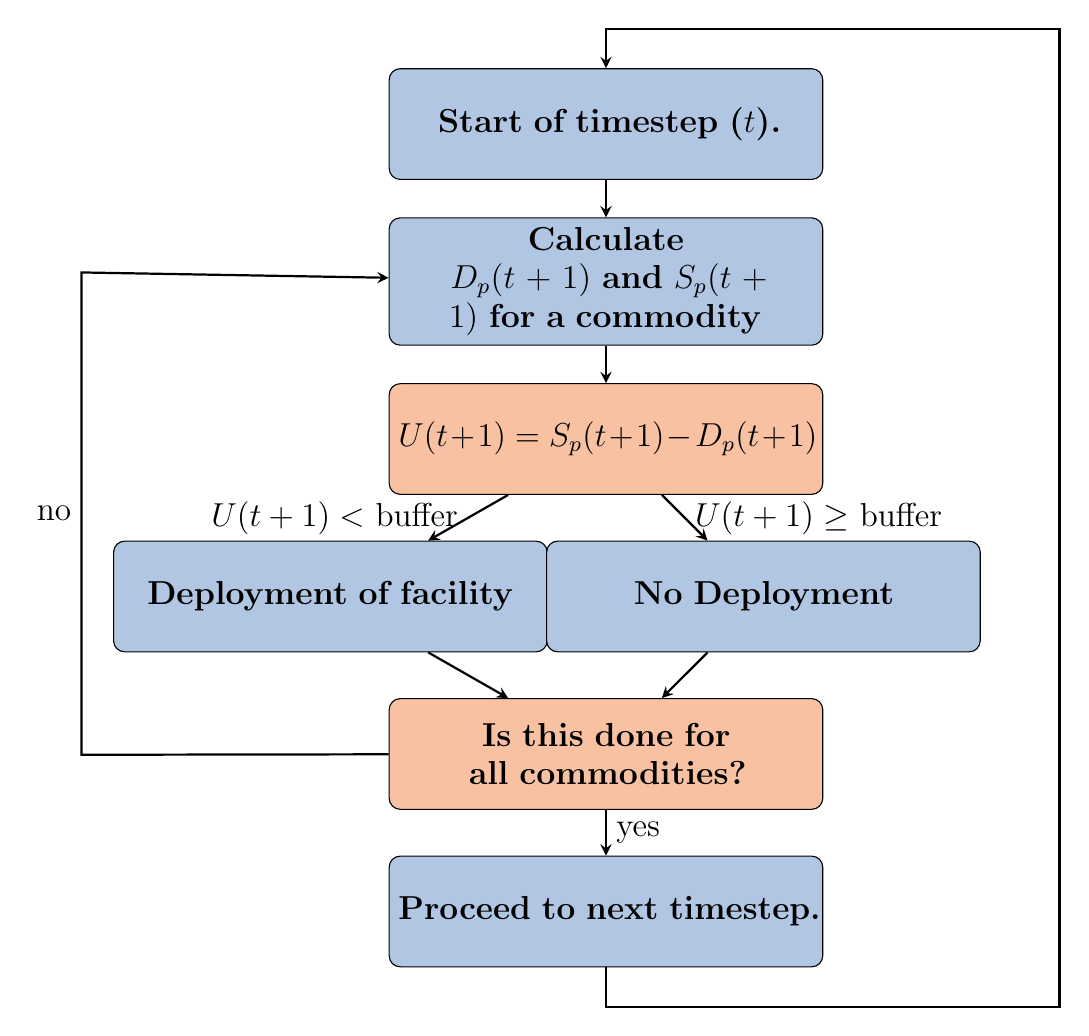
\begin{tikzpicture}[node distance=2cm]
        \tikzstyle{every node}=[font=\large]
        \node (Start) [bblock] {\textbf{Start of timestep ($t$).}};
        \node (Predict) [bblock, below of=Start] {\textbf{Calculate \\ $D_p(t+1)$ and $S_p(t+1)$ for a commodity}};
        \node (IsThere) [oblock, below of=Predict]{\textbf{$U(t+1) = S_p(t+1)-D_p(t+1)$}};
        \node (Deploy) [bblock, below of=IsThere, xshift = -3.5cm]{\textbf{Deployment of facility}};
        \node (NoDeploy) [bblock, right of=Deploy, xshift = 3.5cm]{\textbf{No Deployment} };
        \node (All) [oblock, below of=Deploy, xshift = 3.5cm] {\textbf{Is this done for all commodities?}};
        \node (End) [bblock, below of=All] {\textbf{Proceed to next timestep.}};
        
        \draw [arrow] (Start) -- (Predict); 
        \draw [arrow] (Predict) -- (IsThere);
        \draw [arrow] (IsThere) -- node[anchor=east] {$U(t+1) <$ buffer} (Deploy);
        \draw [arrow] (IsThere) -- node[anchor=west] {$U(t+1) \geq$ buffer} (NoDeploy);
        \draw [arrow] (Deploy) -- (All);
        \draw [arrow] (NoDeploy) -- (All);
        \draw [arrow] (All) -- node[anchor=west] {yes} (End);
        \draw [arrow] (All) -- ([shift={(-3.9cm,0.7cm)}]All.south west)-- node[anchor=east] {no} ([shift={(-3.9cm,-0.7cm)}]Predict.north west)--(Predict);
        \draw [arrow] (End) |-([shift={(3cm,-0.5cm)}]End.south east)-- ([shift={(3cm,0.5cm)}]Start.north east)-|(Start);
        \end{tikzpicture}
        }
        \caption{\deploy logic flow at every timestep in \Cyclus.}
        \label{fig:flow}
    \end{figure}
    \column[t]{3cm}
    \vspace{2cm}
    \begin{align*}
        D_p &= \mbox{Predicted Demand} \\ 
        S_p &= \mbox{Predicted Supply} \\ 
        U &= S_p - D_p 
    \end{align*}
\end{columns}
\end{frame}

\begin{frame}
    \frametitle{\deploy Prediction Methods}
    Non-Optimizing Methods 
    \begin{itemize}
        \item Moving Average (\texttt{ma})
        \item Autoregressive Moving Average (\texttt{arma})
        \item Autoregressive Heteroskedasticity (\texttt{arch})
    \end{itemize}
    Deterministic-Optimizing Methods 
    \begin{itemize}
        \item Fast Fourier Transform (\texttt{fft})
        \item Polynomial Fit (\texttt{poly})
        \item Exponential Smoothing (\texttt{exp-smoothing})
        \item Triple Exponential Smoothing (\texttt{holt-winters})
    \end{itemize}
    Stochastic-Optimizing Methods 
    \begin{itemize}
        \item Auto-Regressive Integrated Moving Averages (\texttt{ARIMA})
    \end{itemize}
\end{frame}
\section{Results}
\begin{frame}
    \frametitle{Breakdown of Results}
    \textbf{The goal is to simulate 4 transition scenarios with fuel cycle facility 
    deployment driven by demand.}  
    \begin{enumerate}
        \item EG01-23 $D(t)=D_0$
        \item EG01-24 $D(t)=D_0+rt$
        \item EG01-29 $D(t)=D_0$
        \item EG01-30 $D(t)=D_0+rt$
    \end{enumerate}

We achieved this by:
\begin{enumerate}
    \item Applying and comparing all prediction methods for each scenario. 
    \item Exploring performance sensitivity to buffer size.
    \item Using the best prediction method and buffer size, demonstrate \deploy 
    deploying reactor and supporting facilities to meet power demand 
    for 4 scenarios. 
\end{enumerate}

\end{frame}

\begin{frame}
    \frametitle{Setting up the Problem}
\textbf{Mass Flow and Facilities in Transition Scenarios: EG01-23 and EG01-29.}

    \begin{figure}[]
        \centering
        \subfigure{\includegraphics[width=0.45\linewidth]{../paper/figures/23flow.pdf}}
        \hspace{1em}
        \subfigure{\includegraphics[width=0.45\linewidth]{../paper/figures/29flow.pdf}}
        \caption{Diagrams with facilities and mass flow of the scenarios EG01-EG23 and EG01-EG29.}
        \label{fig:eg2329}
    \end{figure}
\end{frame}
\subsection{Comparison of Prediction Methods}
\input{compare_prediction}
\subsection{Sensitivity Analysis of Power Buffer Size}
\input{sa}
\subsection{Best Performing Transition Scenarios}
\input{best}
\section{Conclusion}
\subsection{Conclusion}
\begin{frame}
  \frametitle{Conclusion}
        These results demonstrate that by carefully selecting \deploy 
        parameters, we are able to \textbf{effectively automate deployment}
        of reactors and supporting facilities to simulate
        constant and linearly increasing power demand transition scenarios
        for EG01-23, EG01-24, EG01-29, and EG01-30 with minimal 
        power undersupply. 
        \vspace{1em}
        \\
        Not completely eliminating undersupply and under capacity of 
        commodities in the simulation is expected 
        since without time series data 
        at the beginning of the simulation, \deploy takes a few 
        time steps to collect time series data about power demand 
        to predict and start deploying reactor and supporting 
        fuel cycle facilities. 
        
\end{frame}

\begin{frame}
  \frametitle{Future Work}
  \deploy can be used to conduct nuclear fuel cycle \textbf{sensitivity studies}. 
  One of the key issues facing nuclear fuel cycle transition scenario 
  simulations is the presence 
  of idle reactor capacity due to the lack of Pu to fabricate advanced fuels 
  in the simulation. 
  Previously, to conduct sensitivity analysis,  the user would have to manually 
  calculate the deployment scheme for every change in input parameter to avoid 
  idle capacity. 
\end{frame}
\subsection{Future Work}
%\input{future_work}
\input{acks}
%%--------------------------------%%
%%--------------------------------%%
\begin{frame}[allowframebreaks]
  \frametitle{References}
  \bibliographystyle{plain}
  {\footnotesize \bibliography{../paper/bibliography.bib} }

\end{frame}

%%--------------------------------%%


\end{document}



